% TODO: Scrivere discussione dello schema ER finale
\section{Schema E/R finale}
Da una analisi più approfondia si vista la necessità di introdurre delle nuove entità:
\begin{description}
  % TODO: aggiungere immagini entità
\item [Anomalia] con cui si va ad indicare un Sensore non funzionante.
\item [Intervento] per la riparazione di un Sensore non funzionante.
\item [Rilevazione] con cui si va indentificare i dati ralcolti dai sensori.
\end{description}
Caratterizate dalle seguenti relazioni:
\begin{description}
  % TODO: Aggiungere immagini relazioni
\item [Analisi] che va a legare Rivelazioni e Sensore, con cui si va ad indicare i dati racolti dai vari sensori.
\item [Malfunzionamento] che va a legare Sensore ed Anomalia, tramite cui si individuano i sensori non funzionanti.
\item [Risoluzione] che va ad legare Anomalia ed Intervento, azine con cui si va ad riparere un sensore non funzionante.
\end{description}
Nel modello \ref{fig:er-portante} sono riporta le \textbf{cardinalita}specificando il numero minimo e il numero massimo che, le occorrenze, possono assumere in ciascuna associazione, rispetto alle entità. Le cardinalità delle relazioni sono le seguenti: 
\begin{description}
  % TODO: Aggiungere immagini relazioni
\item[Partecipazione] di tipo \textbf{molti a molti (N,N)}; un membro
  dell'equipaggio può essere stato selezionato per la partecipazione
  di diverse missioni spaziali, mentre una missione richiede almeno un
  membro dell'equipaggio.
\item[Stesura] di tipo \textbf{molti a molti (N,N)}; un report può
  essere scritto da molteplici membri dell'equipaggio, mentre un
  membro dell'equipaggio può comporre diversi report.
\item[Report] di tipo \textbf{uno a molti (1,N)}; indica
  l'appartenenza di un report ad un'unica missione, quando invece una
  missione è composta da diversi report che informano dello stato
  della missione man mano.
\item[Risorsa\_1 e Risorsa\_2] entrambe di tipo \textbf{molti a molti
  (N,N)};in quanto una missione ha la possibilità di utilizzare
  molteplici sensori, quando un sensore viene ripiegato per una
  molteplicità di missioni. Analogalmente la relazione è identica per
  l'utilizzo dei robot nelle missioni.
\item[Malfunzionamento] di tipo \textbf{molti a molti (1,N)};
  in quanto quando si presenta un'anomalia, essa si riferisce ad un
  determinato sensore. Invece per i sensori vi è la possibilità di
  trovare diverse anomalie.
\item[Risoluzione] di tipo \textbf{uno a molti (1,N)} quando
  si presenta un'anomalia, un intervento può risolverla. Un intervento
  può essere applicato su diverse anomalie quando hanno la stessa
  causa;.
\item[Eseguito] di tipo \textbf{molti a molti (N,N)}; un
  membro dell'equipaggio può eseguire innumerevoli interventi. Un
  intervento ha la possibilità di essere eseguito, sia da nessun
  membro, che da molteplici membri.
\item[Analisi] di tipo \textbf{uno a molti (1,N)}; una
  rilevazione viene analizzata da un determinato sensore, il sensore
  invece effettua diverse rilevazioni.
\end{description}

\begin{figure}[ht]
  \centering
  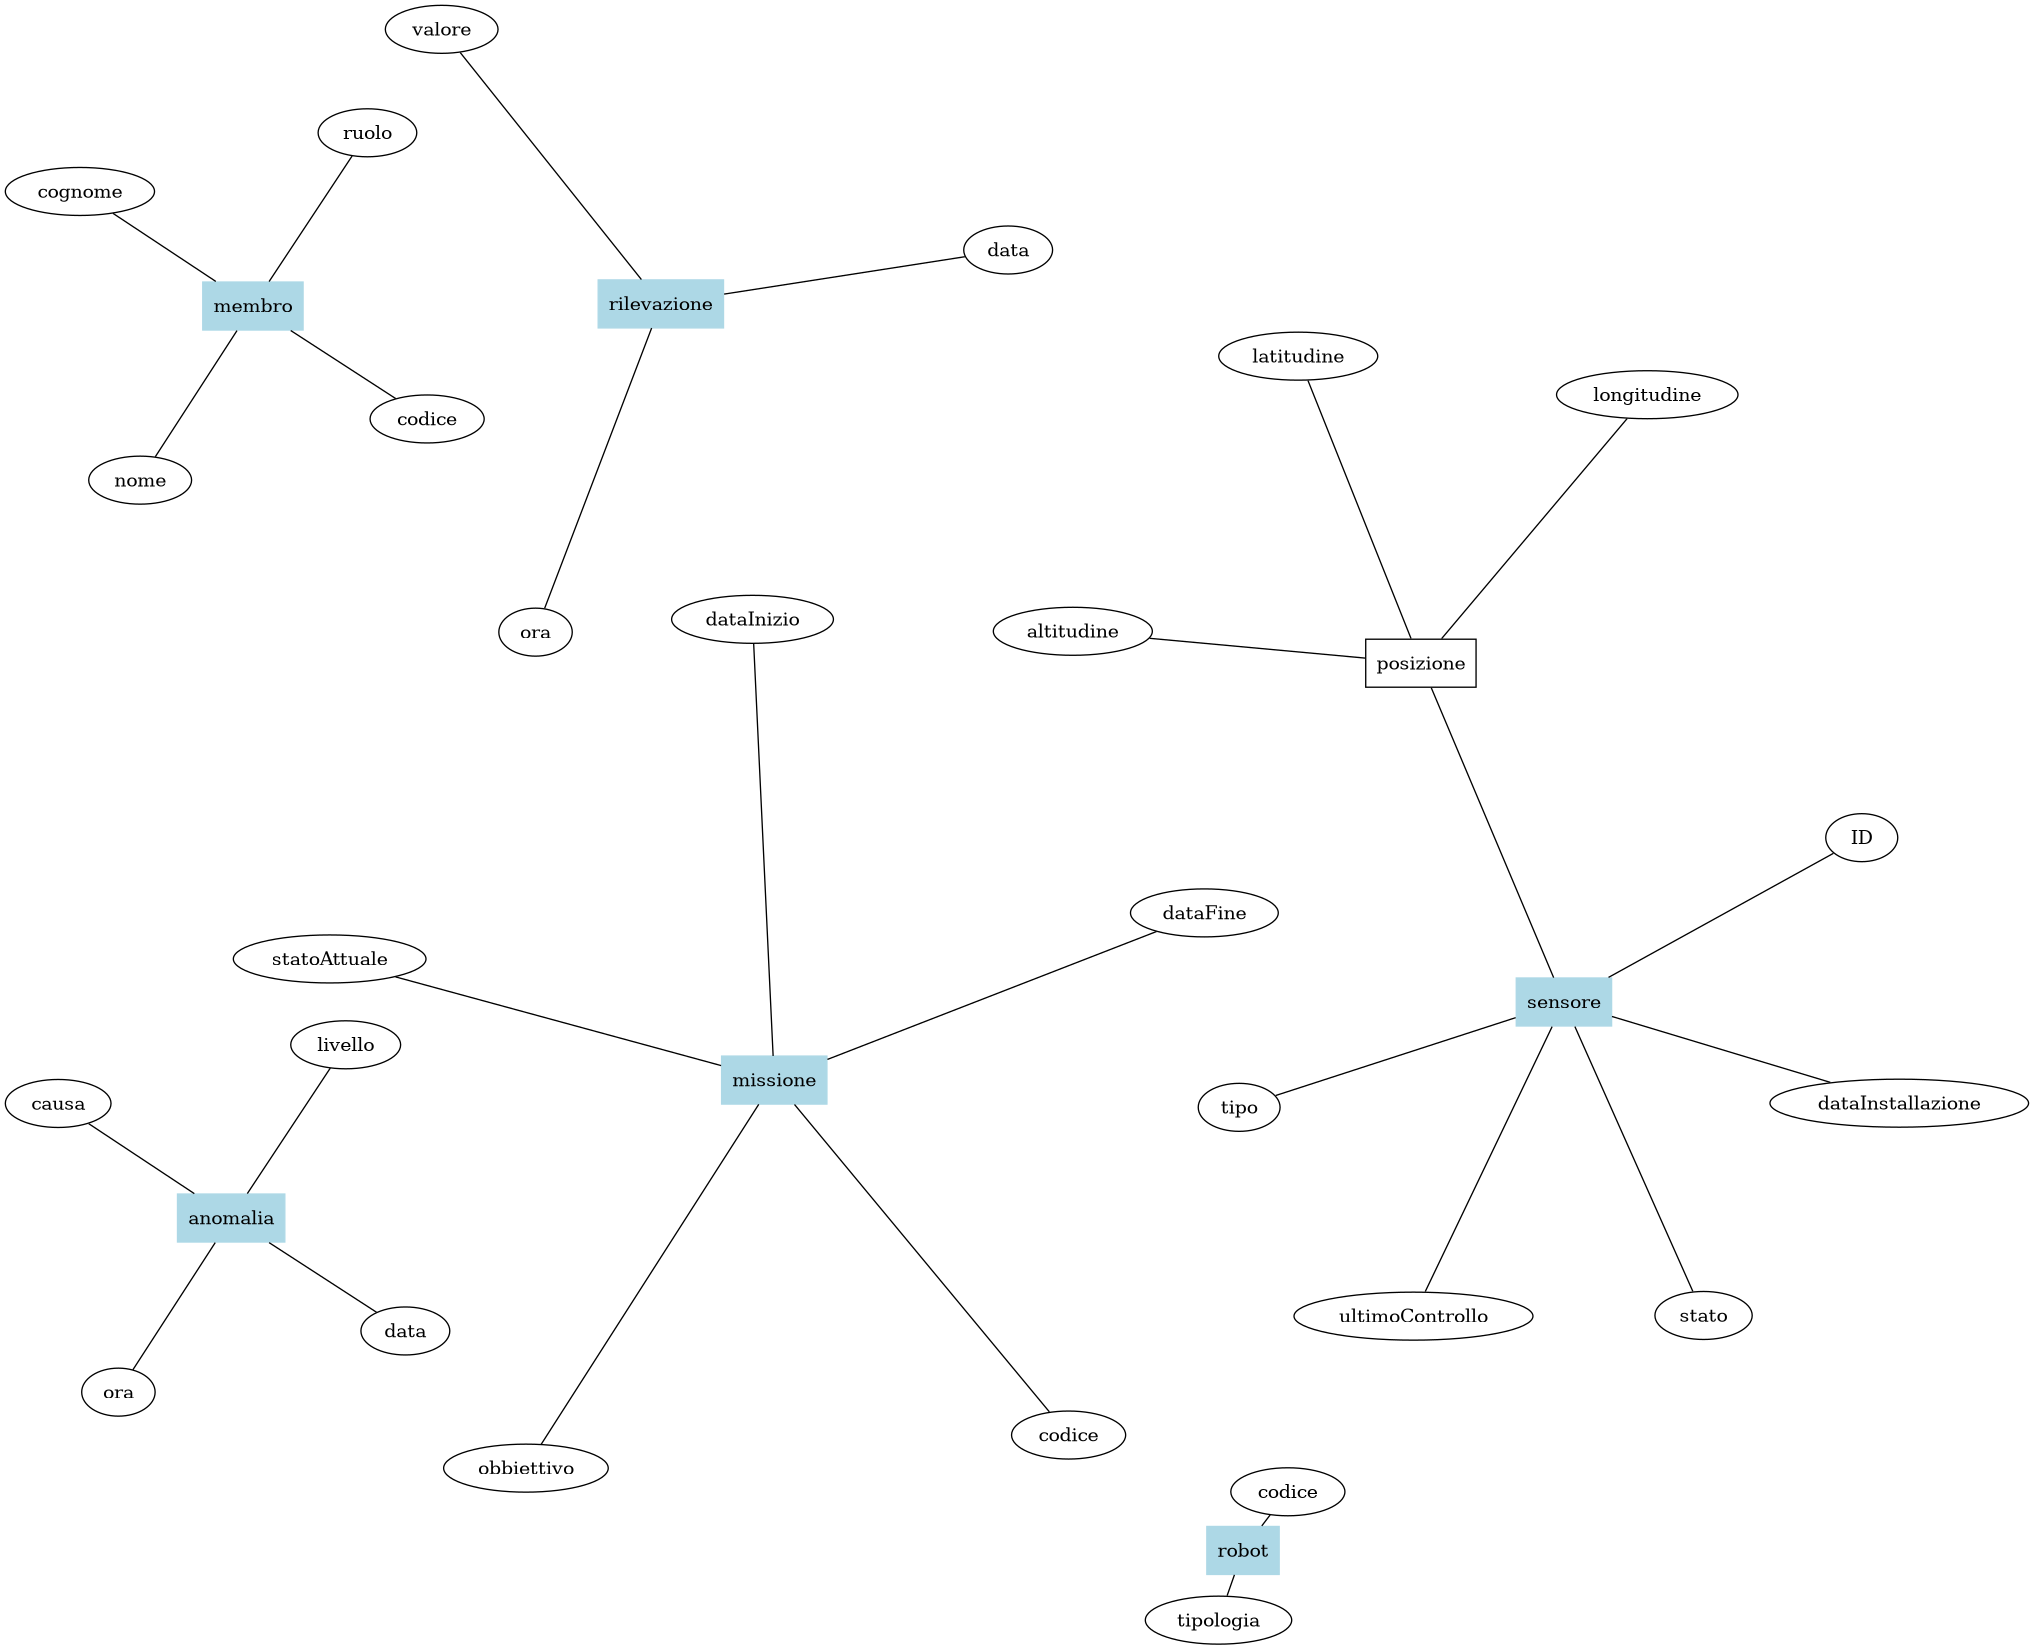
\includegraphics[width=\linewidth]{images/er.png}
  \caption{Modello E/R definitivo per \texttt{ASTRADM}}
  \label{fig:er}
\end{figure}


%%% Local Variables:
%%% mode: LaTeX
%%% TeX-master: "Tesina"
%%% End:
